\documentclass[10pt,t]{beamer}
\usepackage[utf8]{inputenc}
\usepackage[T1]{fontenc}
\usepackage{graphicx}
\usepackage{grffile}
\usepackage{longtable}
\usepackage{wrapfig}
\usepackage{rotating}
\usepackage{amsmath}
\usepackage{textcomp}
\usepackage{amssymb}
\usepackage{capt-of}
\usepackage{hyperref}
\usetheme{default}

% ---------------------------------------------------------------------

\author{L. Larrabee Strow}
\date{\today}
\title{\large The AIRS/CrIS/IASI (and CHIRP) \newline
 Radiative Transfer Algorithms }
\subtitle{\footnotesize{AIRS Science Team Meeting}}
\date{\vspace{0.1in}\footnotesize{September 25, 2019 \vfill}}
\author{C. L. Hepplewhite\inst{1,2}, Sergio DeSouza--Machado\inst{1,2}, L. Larrabee Strow\inst{1,2}}
\institute[UMBC]{\inst{1} UMBC Physics Dept. \and \inst{2}UMBC JCET}
\input beamer_setup
\usetheme{metropolis}
\metroset{titleformat title=allcaps}
\renewcommand{\UrlFont}{\small\tt}
\renewcommand*{\UrlFont}{\footnotesize}
\tolerance=1000
\RequirePackage{fancyvrb}
\DefineVerbatimEnvironment{verbatim}{Verbatim}{fontsize=\footnotesize}
\begin{document}

\maketitle
\addtobeamertemplate{block begin}{
  \setlength{\parsep}{0pt}
  \setlength{\topsep}{3pt plus 2pt minus 2.5pt}
  \setlength{\itemsep}{0pt plus 0pt minus 2pt}
  \setlength{\partopsep}{2pt}
}

% --------------------------------------------------------------------
%%\section{Overview}
%\begin{frame}
%  \frametitle{Overview of talk}
%  \begin{itemize}
%  \item Current status.
%  \item Methods.
%  \item Programmatics.
%  \item Validation and sample results.
%  \item Plans.
    
%  \end{itemize}
%\end{frame}

% ---------------------------------------------------------------------
%%\section{Status}
\begin{frame}
  \frametitle{Status - 1}
  \begin{itemize}
  \item kCARTA calculations of layer-to-space optical depths for all parameters for the 49 and 703 SAF regression profiles for AIRS\_L1C, CrIS FSR and IASI are complete. 
  \item AIRS\_L1C and IASI SARTA update was released May and June this year.
  \item Updated version of AIRS using L1C channel set with SRFs referenced to 10-Sep-2010 drift corrected. 
  \item Spectroscopy based on HITRAN 2016 \& LBLRTM12.8 CO2,CH4 line mixing.
  \item The kCARTA is used to generate TOA radiances to compare directly with SARTA for validation.
  \item CrIS FSR SARTA update for 2019 currently in work.
  
  \end{itemize}
\end{frame}

% ---------------------------------------------------------------------
\begin{frame}
  \frametitle{Status - 2}
  \begin{itemize}
  \item The 2019 SARTA's include the fixed gases, variable \ozone, \water, \cd, \methane, HNO$_3$, \nitrous, SO$_2$, NH$_3$, nonLTE and improved reflected surface thermal. 
  \item AIRS L1c SARTA includes hooks for HDO ($\delta D$), the computation is turned off.
  \item HDO  regression is in progress, regression residuals give $\sim$ 10\% rms, but we think we know how to improve.  What is needed?
  \item SARTA creation for CHIRP will start soon.
  \end{itemize}
\begin{footnotesize}
\vspace{0.1in}
\begin{tabular}{lll}
  \textbf{SARTA Versions} & & \\
  CrIS NSR & HITRAN 2012 & Retired \\
  CrIS FSR & HITRAN 2012 & Will update\\
  AIRS L1b & HITRAN 2008 & Retired \\
  IASI     & HITRAN 2016 & Enhanced SW Continuum\\
  AIRS L1c & HITRAN 2016 & Enhanced SW Continuum \\
  CHIRP    & will be HITRAN 2016 & Enhanced SW Continuum
\end{tabular}
\end{footnotesize}
%  \begin{itemize}
    % \item Build Matrix
    % \item CrIS NSR HITRAN2012
    % \item CrIS FSR HITRAN2012
    % \item AIRS L1B HITRAN2008
    % \item AIRS\_L1C HITRAN2016
    % \item IASI HITRAN2016
    % \end{itemize}
  

\end{frame}

% ---------------------------------------------------------------------
%\section{Methods}
%\begin{frame}
%  \frametitle{}
%  \begin{itemize}
%  \item 
%  \item 
%  \item 
%  \item 
%  \item 
    
%  \end{itemize}
%\end{frame}

% ---------------------------------------------------------------------
%\section{Programmatics}
%\begin{frame}
%  \frametitle{}
%  \begin{itemize}
%  \item 
%  \item 
%  \item 
%  \item 
%  \item 
    
%  \end{itemize}
%\end{frame}

% ---------------------------------------------------------------------
%\section{Results}
%\begin{frame}
%  \frametitle{}
%  \begin{itemize}
%  \item 
%  \item 
%  \item 
%  \item 
%  \item 
    
%  \end{itemize}
%\end{frame}

% ---------------------------------------------------------------------
\begin{frame}
  \frametitle{Results - IASI}
  \begin{center}
    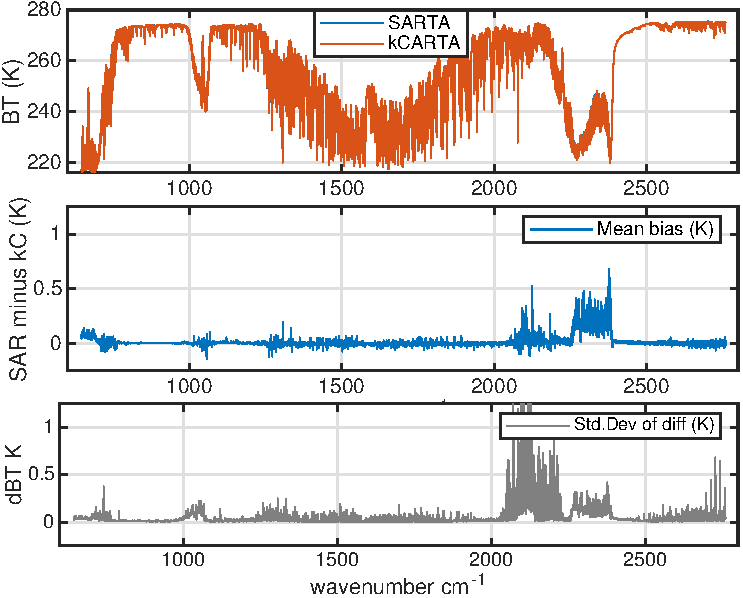
\includegraphics[width=0.9\linewidth]{./Figs/Pdf/kc_sar_iasi_mean_bias_stdv_sea_6angs_aslp.pdf}
  \end{center}
      
 \end{frame}

% ---------------------------------------------------------------------
\begin{frame}
  \frametitle{IASI:  Parameterization Error Correlations}
  \begin{center}
    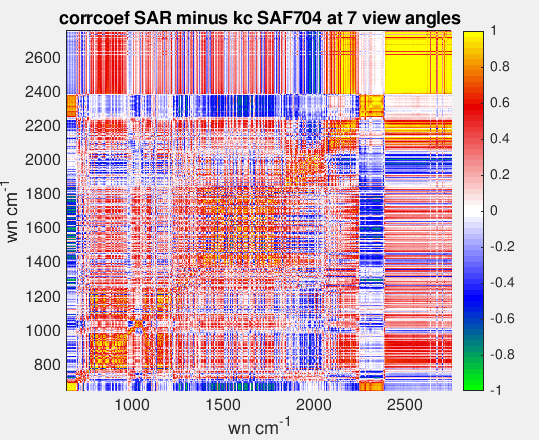
\includegraphics[width=0.8\linewidth]{./Figs/Png/plot1.png}
  \end{center}

This does not include correlations due to spectroscopy errors.
  
 \end{frame}

% ---------------------------------------------------------------------
\begin{frame}
  \frametitle{Results - AIRS\_L1C}
  \begin{center}
    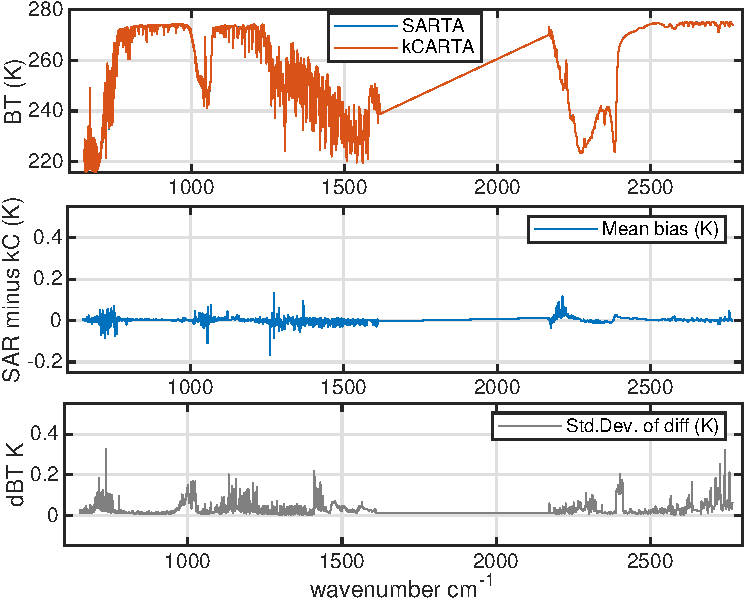
\includegraphics[width=0.9\linewidth]{./Figs/Pdf/kc_sar_airs_l1c_mean_bias_stdv_sea_6angs_aslp.pdf}
  \end{center}
      
 \end{frame}

% ---------------------------------------------------------------------
\begin{frame}
  \frametitle{AIRS:  Parameterization Error Correlations}
  \begin{center}
    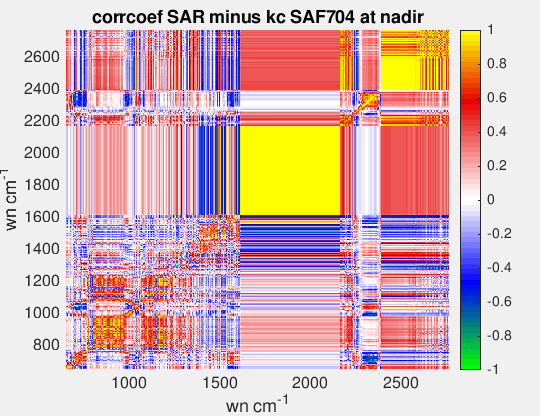
\includegraphics[width=0.9\linewidth]{./Figs/Png/plot6_wavenumber_sorted.png}
  \end{center}
      
 \end{frame}

% ---------------------------------------------------------------------
\begin{frame}
  \frametitle{AIRS\_L1C Mean \& Std. Dev Errors vs angle}

  \begin{center}
    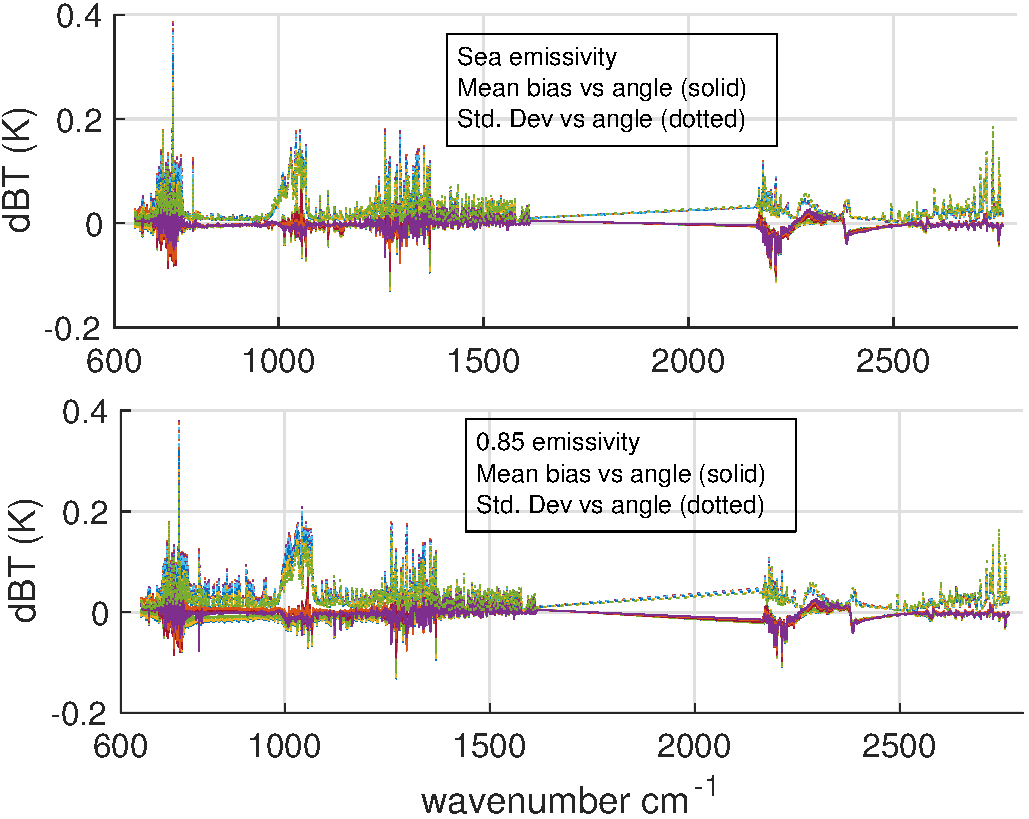
\includegraphics[width=0.9\linewidth]{./Figs/Pdf/kc_sar_airs_l1c_mean_stdv_emiss_vs_angle_v2.pdf}
  \end{center}
  
  \end{frame}


  \begin{frame}
    \frametitle{Standard Deviations}
    \begin{itemize}
    \item Std. deviations are over 49 fitting profiles and 6 secant angles
    \item The fitting profiles span global variability very nicely
    \item Std. Dev. will be smaller with a global average profile data set
    \end{itemize}
  \end{frame}

\begin{frame}{New Spectroscopy (other than HITRAN)}
\begin{block}{New Shortwave Continuum (Hartmann)}
\begin{itemize}
\item Important new physics, \nitrogen-\water and \cd-\water continuum
\item Affects temperature sounding region
\item Existing RTAs have dependence on \water wrong!  Either using quadratic on none.
\item Hartmann has published these improvements (GRL 2018)
\item We have partially validated them and included them in new RTA
\end{itemize}
\end{block}
\end{frame}

\begin{frame}[label={sec:org3f23098}]{New Continuum Characteristics}
\begin{columns}
\begin{column}{0.55\columnwidth}
\begin{block}{\small \(\Delta\) B(T) a 2400 \wn vs column water}
\begin{center}
\includegraphics[width=\linewidth]{./Figsh/co2_wat_n2_wat_2400_cm_vs_mmw.pdf}
\end{center}
\end{block}
\end{column}

\begin{column}{0.55\columnwidth}
\begin{block}{\small Spectral effects for 20 cm water}
\begin{center}
\includegraphics[width=\linewidth]{./Figsh/co2_wat_n2_wat_spectrum_mean_fitting.pdf}
\end{center}
\end{block}
\end{column}
\end{columns}
\end{frame}

\begin{frame}
  \frametitle{Conclusions}
  \begin{itemize}
  \item SARTA AIRS L1c delivered
  \item But, might be better to just jump to CHIRP radiances and CHIRP RTA??
  \item Hope to finalize HDO soon, but would like input on accuracy needs
  \item Will be doing more validation on Hartman continuum, quick look very encouraging
  \end{itemize}
\end{frame}


% \begin{frame}[label={sec:org3861167}]{\nitrogen-\water and \cd-\water continuum: Sonde Validation}
% \vspace{-0.2in}
% \begin{columns}
% \begin{column}{0.55\columnwidth}
% \begin{block}{Full Spectrum}
% \begin{center}
% 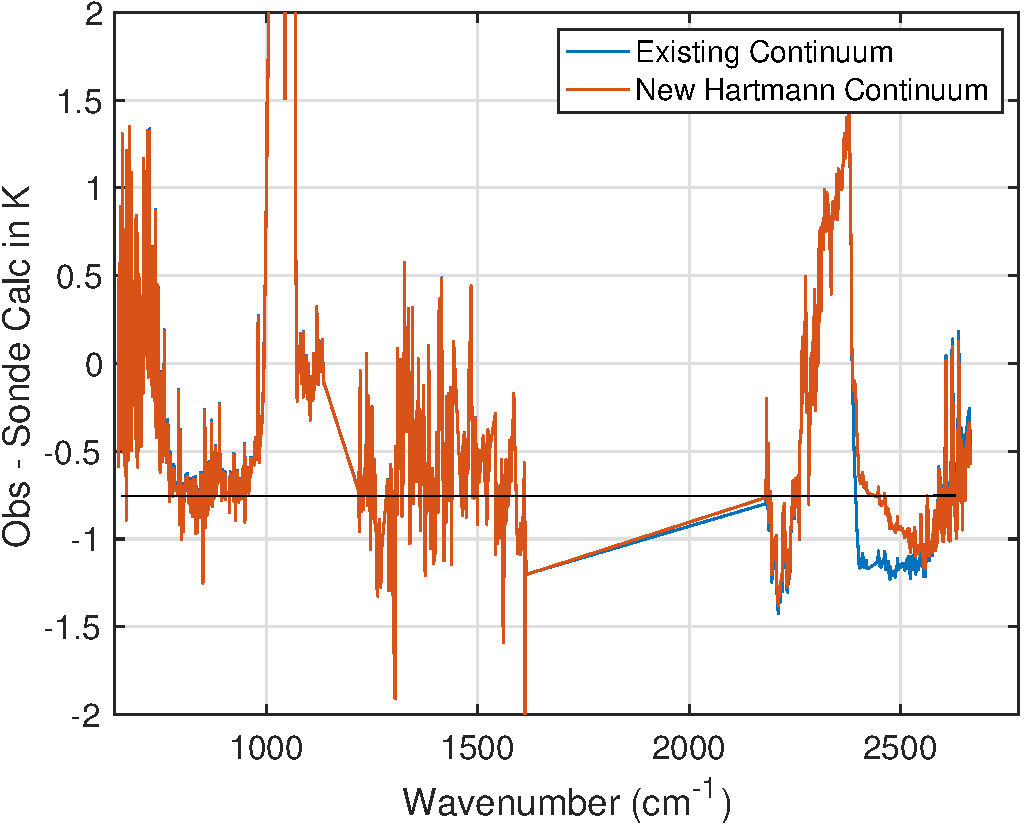
\includegraphics[width=\linewidth]{./Figs/hartman_full.pdf}
% \end{center}
% \end{block}
% \end{column}
% \begin{column}{0.55\columnwidth}
% \begin{block}{Shortwave Zoom}
% \begin{center}
% 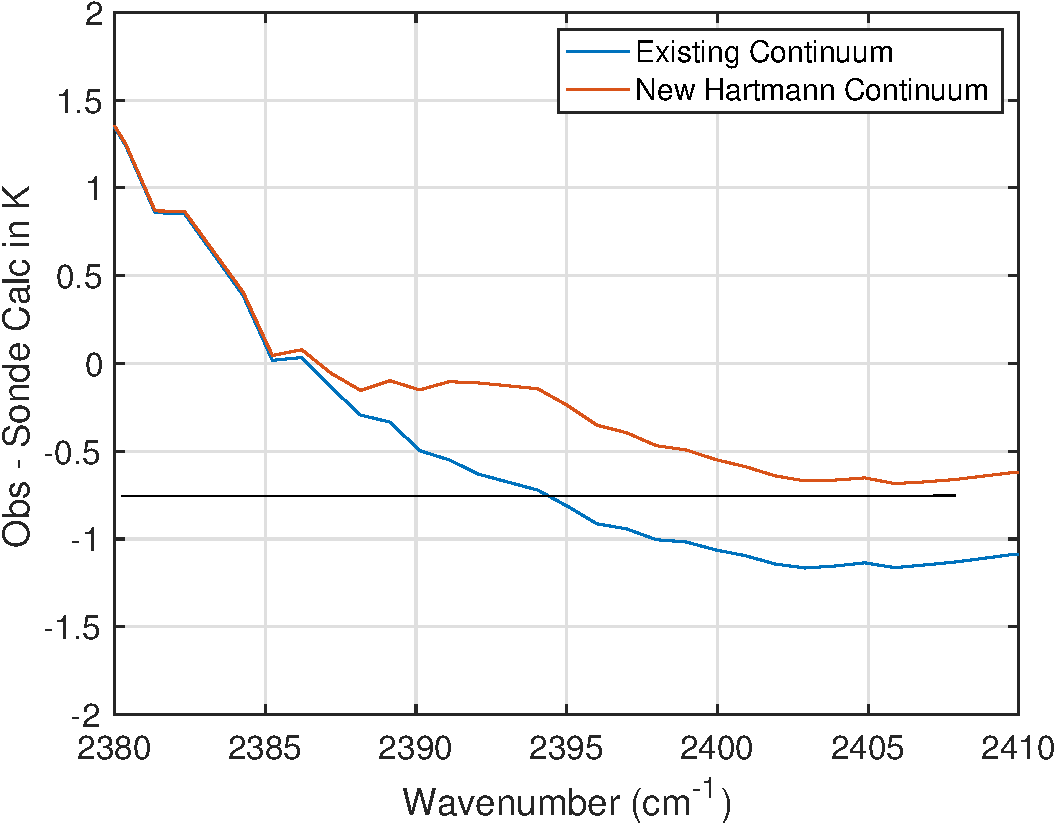
\includegraphics[width=\linewidth]{./Figs/hartman_2400.pdf}
% \end{center}
% \end{block}
% \end{column}
% \end{columns}

% \begin{itemize}
% \item \small Better agreement with thermal window SST near band-head
% \item \small Not important for low-humidity conditions (not shown)
% \end{itemize}
% \end{frame}


  


%  \section{Plans}
%\begin{frame}
%  \frametitle{Current and future Plans}
%  \begin{itemize}
%  \item 
%  \item 
%  \item 
%  \item 
%  \item 
    
%  \end{itemize}
%\end{frame}

% ---------------------------------------------------------------------

\end{document}

%%% Local Variables:
%%% mode: latex
%%% TeX-master: t
%%% End:
